%%% LaTeX Template
%%% This template can be used for both articles and reports.
%%%
%%% Copyright: http://www.howtotex.com/
%%% Date: February 2011

%%% Preamble
\documentclass[paper=a4, fontsize=11pt]{scrartcl}	% Article class of KOMA-script with 11pt font and a4 format

\usepackage[margin=0.7in]{geometry}
\setcounter{secnumdepth}{4}

\usepackage[english]{babel}															% English language/hyphenation
\usepackage[protrusion=true,expansion=true]{microtype}				% Better typography
\usepackage{amsmath,amsfonts,amsthm}										% Math packages
\usepackage[pdftex]{graphicx}														% Enable pdflatex
%\usepackage{color,transparent}													% If you use color and/or transparency
\usepackage[hang, small,labelfont=bf,up,textfont=it,up]{caption}	% Custom captions under/above floats
\usepackage{epstopdf}																	% Converts .eps to .pdf
\usepackage{subfig}																		% Subfigures
\usepackage{booktabs}																	% Nicer tables


%%% Advanced verbatim environment
\usepackage{verbatim}
\usepackage{fancyvrb}
\DefineShortVerb{\|}								% delimiter to display inline verbatim text


%%% Custom sectioning (sectsty package)
\usepackage{sectsty}								% Custom sectioning (see below)
\allsectionsfont{%									% Change font of al section commands
	\usefont{OT1}{bch}{b}{n}%					% bch-b-n: CharterBT-Bold font
%	\hspace{15pt}%									% Uncomment for indentation
	}

\sectionfont{%										% Change font of \section command
	\usefont{OT1}{bch}{b}{n}%					% bch-b-n: CharterBT-Bold font
	\sectionrule{0pt}{0pt}{-5pt}{0.8pt}%	% Horizontal rule below section
	}


%%% Custom headers/footers (fancyhdr package)
\usepackage{fancyhdr}
\pagestyle{fancyplain}
\fancyhead{}														% No page header
\fancyfoot[C]{\thepage}										% Pagenumbering at center of footer
\renewcommand{\headrulewidth}{0pt}				% Remove header underlines
\renewcommand{\footrulewidth}{0pt}				% Remove footer underlines
\setlength{\headheight}{13.6pt}

%%% Equation and float numbering
\numberwithin{equation}{section}															% Equationnumbering: section.eq#
\numberwithin{figure}{section}																% Figurenumbering: section.fig#
\numberwithin{table}{section}																% Tablenumbering: section.tab#
\usepackage[parfill]{parskip}
\usepackage{float}
\usepackage{graphicx}

%%% Title	
\title{ \vspace{-1in} 	\usefont{OT1}{bch}{b}{n}
		\huge \strut An Overview of the Development of Indirect Inelastic Data Analysis in Mantid\strut \\
}
\author{ 									\usefont{OT1}{bch}{m}{n}
        Samuel Jackson\\		\usefont{OT1}{bch}{m}{n}
		ISIS Facility\\	\usefont{OT1}{bch}{m}{n}
        STFC Rutherford Appleton Laboratory\\
        \texttt{samuel.jackson@stfc.ac.uk}
}
\date{\today}

%%% Begin document
\begin{document}
\maketitle
\clearpage
\tableofcontents
\section{Introduction}
Mantid (http://www.mantidproject.org) is an open source, cross platform framework for the analysis of Neutron and Muon scattering data. The project is primarily written in C++ with a Python API. The project includes a GUI based off of the QtiPlot project and primarily written using the Qt library.

Mantid aims to provide a single platform for neutron and muon scattering data analysis to all facilities across the world. It is developed by two teams of developers, one based at the ISIS facility at Rutherford Appleton Laboratory UK, the other at the SNS facility at Oakridge USA. Recently additional partners from the ILL and PSI have also contributed.

The project is currently still under heavy development and provides regular incremental releases for evaluation and feedback from instrument scientists and users in general and is therefore constantly evolving with each release. Until recently, Mantid operated on a three month release cycle. This has now been changed to so that the project releases every four months, with a longer emphasis on the testing and integration phase of development.

Up until now the indirect inelastic section of Mantid has largely been based off of the the existing MODES application which in turn was based on OpenGenie\cite{wshowells2010}. The majority of the functionality has now been integrated into the Mantid framework in one form or another and we are now beginning to reach a point where we can expand the existing functionality further.

This document aims to give an overview of the current stage of development for the indirect inelastic section of the application as it currently exists in as much detail as possible to provide a historical snapshot of the progress so far. The remainder of the document then provides a weak outline of suggested directions for further development in the future.

%\section{A Brief Introduction to Neutron Scattering}
%Neutron scattering experiments are used to probe the structure of materials at a fundamental level. The results of such experiments can be used to learn a great deal about the internal structure of a sample and how it can behave under different conditions. In a neutron scattering experiment, a beam of neutrons is produced at a source (such as the one provided by ISIS) and directed to the various instruments attached to the beam line. These neutrons then scatter from the sample placed in the instrument. The angle and energy at which scattered neutrons are detected can then be used to deduce the structure and dynamics of the sample.
%
%There are two main types of neutron scattering: elastic and inelastic. Elastic scattering is the special case when the final energy is equal to the incident energy and there is no energy transfer and the kinetic energy of the incident neutrons remain unchanged. Inelastic scattering is the more general case where some change in the kinetic energy of the incident neutron occurs and is useful for measuring the vibrations of atoms\cite{rpynn2008}.

\section{Data Reduction with Mantid}
Mantid provides a collection of graphical user interfaces to specialised indirect inelastic data reduction routines under the menu \textit{Interfaces \textgreater Indirect}. The majority of these routines are based on or directly ported from the MODES3 and the Iris Data Analysis (IDA) package\cite{wshowells2010}. As such, the core of the functionality of these routines has mostly remained the same, but the implementation has changed. This section outlines the current development of each of the interfaces and routines available.

\subsection{Theory}
\mbox{ }\\
\begin{figure}[H]
\centering
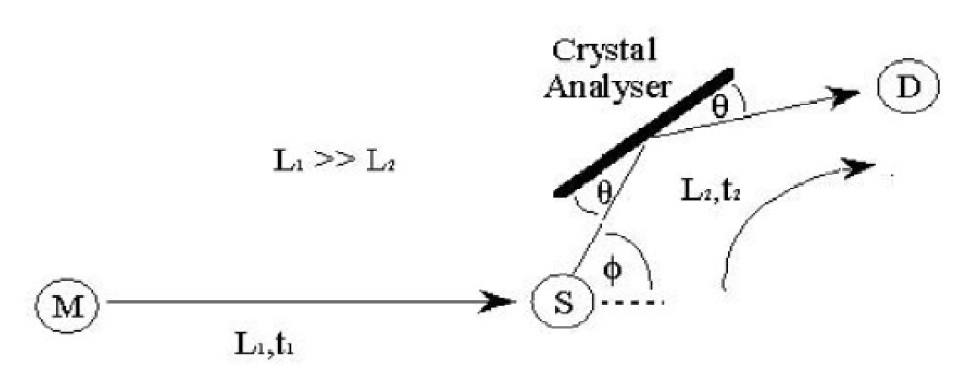
\includegraphics[width=0.7\textwidth]{img/instrument-diagram.png}
\caption{Diagram of the basic principle of an inelastic neutron scattering experiment. M is the moderator, S is the sample, and D is the detector \cite{smukhopadhyay2014}}
\label{fig:instrument-setup}
\end{figure}

In order to convert the raw data collected from the instrument from time of flight measurements to energy transfer the routine uses known parameters about the instrument as illustrated in figure \ref{fig:instrument-setup}. The final energy detected by a detector can be written in terms of a neutron's mass ($m_{n}$) and velocity ($v$) from the sample to the detector:

\begin{equation}
E_f = \frac{1}{2}m_{n}v^2 = \frac{1}{2}m_{n} ( L_2 / t_2 ) ^2 
\end{equation}

Which can also be written in terms of the distance between sample and detector ($L_2$) and the time of flight $t_2$. To calculate the transfer of energy knowledge of the flight path between the moderator and sample ($L_1$) and the time of flight over this distance ($t_1$) can be used to calculate the incident energy using equation above. The transfer of energy is then simple the difference between incident and final energy:

\begin{equation}
\Delta E = E_i - E_f = \frac{1}{2}m_n[(L_1 / t_1-t_2)^2 - (L_1/t_2)^2]
\end{equation}

This is the fundamental principle behind the reduction routine described in the following section.

\subsection{Implementation}
The Convert to Energy interface provides the initial entry point for data into Mantid for indirect inelastic instruments. The functionality of this interface is currently also shared with the direct instruments, although a separation of the interfaces is planned in future releases.

\subsubsection{Energy Transfer}
\label{sec:energy-transfer}
The Energy Transfer tab on the Convert To Energy interface is the starting point for data reduction. The energy transfer routine, as the name suggests, is used to convert the a raw file representing a sample run from the raw TOF measurement to units of energy transfer and also performs general preprocessing of the data to get it ready for analysis.

The structure of the underlying energy transfer reduction routine is based on the older Mantid concept of a Reducer class which has since been superseded by the concept of algorithms and work-flow algorithms. The Reducer class is contains a list of ReductionSteps, which represents a single logical operation to be carried out as part of the reduction. ReductionSteps themselves just call Mantid algorithms and contain the actual implementation details of the operation to be performed.

\begin{figure}[H]
\centering
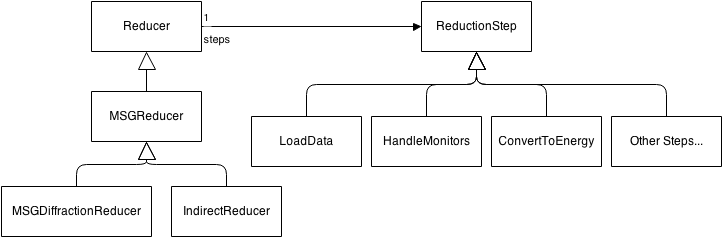
\includegraphics[width=1\textwidth]{img/uml/class_diagrams/Reducer_structure.png}
\caption{Diagram showing the class structure for the inelastic reducers and accompanying reduction steps.}
\label{fig:reducer-structure-diagram}
\end{figure}

Figure \ref{fig:reducer-structure-diagram} shows the class structure of indirect reducers and a subset of the reduction steps that are defined for inelastic energy reduction. In indirect data analysis we have two concrete reducer objects. One for energy conversion (IndirectReducer) and one for diffraction reduction (MSGDiffractionReduction). This section will just focus on the IndirectReducer. For discussion on diffraction reduction see section \ref{subsec:indirect-diffraction}. 

The IndirectReducer object defines what steps should be executed as part of a reduction work-flow and is the point at which the parameters gather from the user interface are passed to the program. After setting up the each reduction step with the relevant parameters, the reducer then iterates over the list of steps and executes each one in turn on the sample run to be reduced. Reducer objects also have the option to define a preprocessing function which is only executed once regardless of the number of runs being processed. The MSGReducer, which is the superclass of both the IndirectReducer and the MSGDiffractionReducer, uses this to execute the loading step to get the sample run(s) to be reduced into memory before continuing with the rest of the reduction on a per run basis.

\begin{figure}[H]
\centering
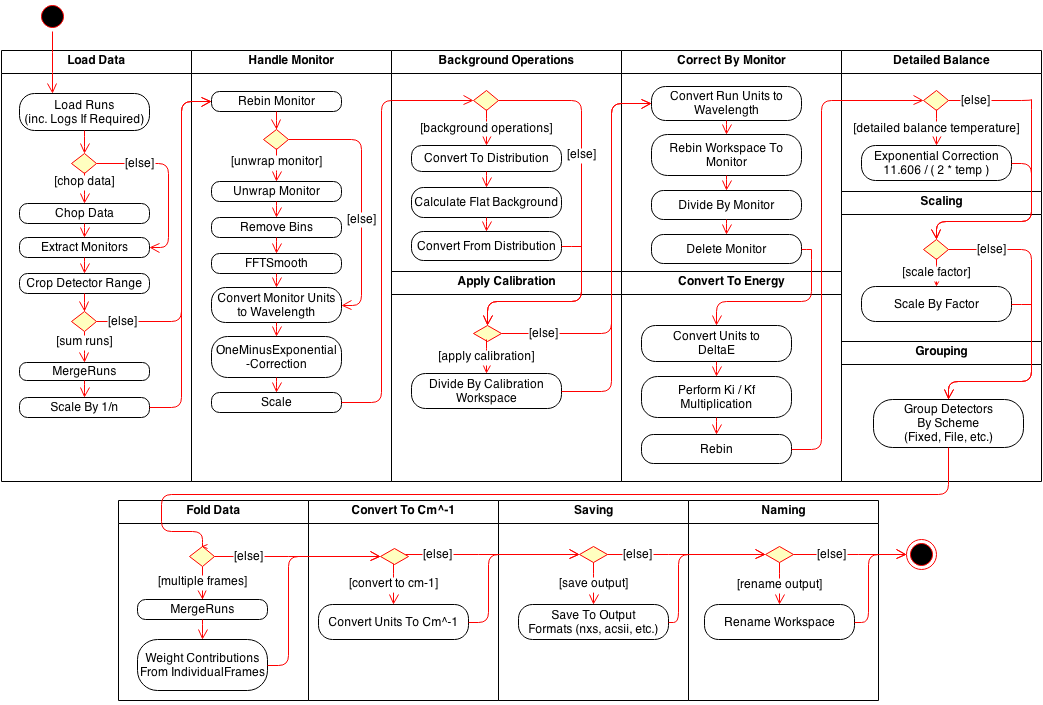
\includegraphics[width=1\textwidth]{img/uml/activity_diagrams/EnergyTransfer_activity.png}
\caption{Activity diagram showing the flow of execution for energy transfer reduction in release 3.2.}
\label{fig:c2e-energy-transfer-activity-diagram}
\end{figure}

The steps involved in energy transfer reduction are shown in activity diagram \ref{fig:c2e-energy-transfer-activity-diagram} along with the major operations performed within each step and the flow of the execution of the reduction. The responsibility of each of the steps are as follows:

\begin{itemize}
\item \textbf{Load Data} - The load data step loads each individual sample runs from file using the correct loader for the currently selected instrument. If the option is selected, it will also attempt to load the logs for the runs as well. If the current instrument has the parameter Workflow.ChopDataIfGreaterThan defined as in its instrument parameter file (IPF), the reduction step splits the data into multiple frames using the ChopData algorithm. The routine will then extract the monitor from the loaded workspace and crop the workspace to the desired detector range. If the sum option is checked the runs will be merged into a single workspace and averaged, otherwise subsequent steps are executed on each run individually.

\item \textbf{Handle Monitor} - Next the reducer prepares the monitors for correction later. This involves rebinning the monitor according to the step size defined the the IPF If. Next it will unwrap the monitor, if required, using the UnwrapMonitors algorithm to convert the workspace to have common bins within the maximum wavelength range given a reference flightpath between source, sample and first detector. It then tidies up the monitor by removing the bin at the joining wavelength and smooths it Using FFTSmooth. Finally it converts the units of the workspace to wavelength, performs an exponential correction for the thickness, attenuation and area of the monitor and scales it if a scaling factor is defined in the IPF.

\item \textbf{Background Operations} - This step simply calculates a flat background for the detectors data if parameters are defined for the background range and calculates the mean of the bins in this range before dividing by the width of the x range.

\item \textbf{Correct By Monitor} - The reducer then corrects the workspace by the preprocessed monitor by converting the units to wavelength then rebinning it to and dividing it by the monitor.

\item \textbf{Convert To Energy} - The conversion of the workspace to units of energy is then performed and multiplied by ki / kf , to transform the differential scattering cross section into a dynamic structure factor. The workspace is then rebinned according to the user defined rebin string.

\item \textbf{Detailed Balance} - The detailed balance step converts performs an exponential correction on the data if a temperature parameter was defined by the user.

\item \textbf{Scaling} - This step will scale the workspace by an arbitrary factor supplied by the user.

\item \textbf{Fold Data} - If the data was split into multiple frames during the loading step, the fold data step is performed. The individual frames are merged back into a single workspace and the workspace is scaled by averaging the contributions of each individual frame across the x range.

\item \textbf{Convert To $Cm^{-1}$} - If the option was selected, the workspace is convert to units of wavenumber.

\item \textbf{Saving} - If any save options were selected, the reduced workspace is saved in the desired format.
\item \textbf{Naming} - Finally, the reduced workspace is renamed according to the instrument-analyser-refection convention used in Mantid indirect inelastic.
\end{itemize}

\subsubsection{Calibration}
The calibration section of the convert to energy interface can be used to create calibration and resolution files using vanadium sample runs which can be used as part of data reduction and analysis. Calibration workspaces are generated by creating an executing a single reduction step object  (without creating a reducer object) called CreateCalibrationWorkspace. The procedure for generating a single calibration step is to load the runs, and if there is more then one of them merge them and scale the output workspace by a factor of $1/\,number\,of\,runs$. It then calculates a flat background based on a background range supplied by the user. The routine then integrates over the peak range (again, supplied by the user) and scales the resulting workspace. An activity diagram for the routine is shown in figure \ref{fig:c2e-calibration-activity-diagram}.

\begin{figure}[H]
\centering
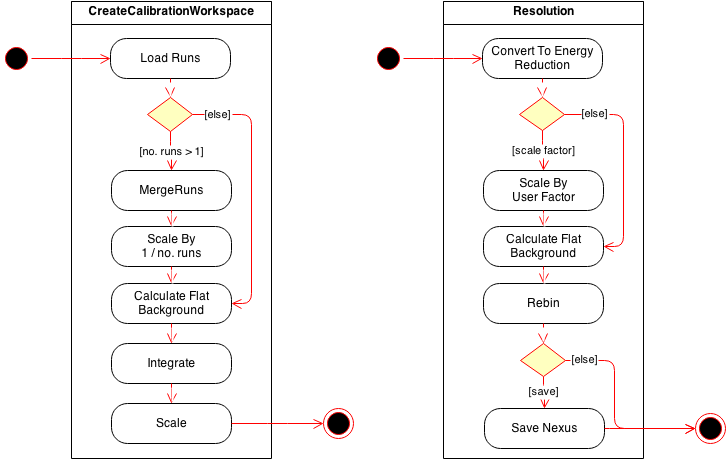
\includegraphics[width=0.6\textwidth]{img/uml/activity_diagrams/Calibration_activity.png}
\caption{Activity diagram showing the major steps of execution performed when creating a calibration and resolution workspace.}
\label{fig:c2e-calibration-activity-diagram}
\end{figure}

As mentioned, the calibration interfaces can also create resolution files for later use in data analysis. This routine, like many within the indirect section of many, is separate from the reducer-reduction step  framework and just a python function which is executed with parameters supplied from the interface. To create the resolution file, the routine first takes the vanadium run supplied on the calibration interface and converts it to energy using the energy transfer reducer described in section \ref{sec:energy-transfer}, but sets the detector mapping use all detectors and will sum multiple run if multiple runs are used. It then, like calibration, calculates a flat background from a range supplied by the user, rebins it according to the parameters specified for the instrument, and optionally saves the workspace to file.

\subsubsection{Diagnostics}
The diagnostics routine provides an integration on a run over a specified time-of-flight range. This routine loads the raw file and a calibration file (if requested) and integrates the resulting workspaces. If two ranges are requested, the second range is used to calculate a flat background and remove this from the data before integrating. Finally, the integrated workspace is then transposed to make it easier to visualise.

\subsubsection{Transmission}

\subsubsection{$S(Q,w)$}
In this interface, reduced files created as part of an energy transfer reduction can be converted to $S(Q,w)$. The Mantid framework has a collection of three algorithms that are used to convert a workspace from energy transfer to $S(Q,w)$ depending on the choice of rebinning to use. The mapping between $S(Q,w)$ algorithms and the rebin types are given in table \ref{table:sofqw-algorithms}. The code running an $S(Q,w)$ conversion is entirely contained within the Indirect interface where it dynamically builds a string of python code that is then executed. Optionally, the user many rebin the workspace in energy before hand. In this case, the routine simply calls the rebin algorithm with given parameters.

\begin{table}[H]
\begin{center}
\begin{tabular}{ c c}
Rebin Type & Algorithm Used \\ \hline
Centre & SofQW \\ 
Parallelepiped & SofQW2 \\ 
Parallelepiped / Fractional Area & SofQW3 \\ 
\end{tabular}
\caption{Table showing the relationship of rebin types to SofQW algorithms}
\label{table:sofqw-algorithms}
\end{center}
\end{table}

\subsubsection{$S(Q,w)$ Moments}
This is a new addition in Mantid 3.2 and provides a simple routine for calculating the first five statistical moments of an $S(Q,w)$. This is implemented as a standard Mantid algorithm (SofQWMoments) which is created and called from the interface though the algorithm manager and produces a group workspace with one workspace for each moment for every detector which has been transposed in order to make visualisation of the workspace easier.


\subsection{GUI}
Figure \ref{fig:c2e-class-diagram} shows the class structure of the indirect convert to energy. Note that for clarity only the more important methods and attributes are shown as part of the class diagram. The Convert to Energy window (for both direct and indirect instruments) inherits from Mantid's generic UserSubWindow class which provides the basic functionality required to render a sub window within the application and also provides some useful helper methods such as the ability to execute a string as a python script.

The ConvertToEnergy class itself contains the code which is shared between both direct and indirect versions of the interface. It is responsible for the loading the appropriate instrument definition files as the user selects an instrument, swapping between the indirect and direct interfaces depending on the geometry of the selected instrument, and handling the major user actions such as clicking the run energy transfer and help buttons.

\begin{figure}[H]
\centering
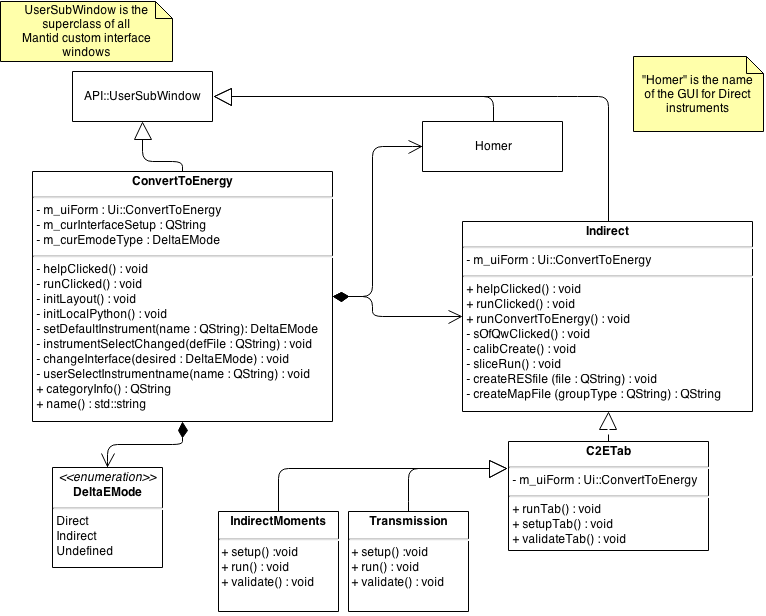
\includegraphics[width=0.8\textwidth]{img/uml/class_diagrams/C2E_structure.png}
\caption{Class diagram showing the structure of the Indirect Convert To Energy GUI in release 3.2.}
\label{fig:c2e-class-diagram}
\end{figure}

ConvertToEnergy is composed with two classes called Homer and Indirect that handle the functionality of direct and indirect geometry instruments respectively. In previous releases of Mantid the Indirect class contained all of the GUI code for every tab on the Indirect Convert To Energy interface. This is no longer the case in more recent versions of Mantid which have moved towards a more modular class structure.

As of release 3.2, the Indirect class contains the GUI code for the Energy Transfer, Calibration, Diagnostics, and S(Q,w) tabs. For each of these tabs there are corresponding methods (which are inconsistently named) to validate the user's input for that tab and run the appropriate routine. The specifics of each of these routines is outlined in the following sections. In order the execute the required routine, the GUI code for a particular tab builds a string which represents an executable python script complete with the options collected from the interface that can be executed using the runPythonCode() method inherited from UserSubWindow.

The actual design of the GUI is stored in a separate xml file that was created using Qt Designer and is used to produce a dynamically generated class for the interface at compile time which includes all the interface widgets for ConvertToEnergy. The ConvertToEnergy, Homer, and Indirect classes each have a reference to a copy of this interface object which they can query at runtime. The ConvertToEnergy class is responsible for adding and removing the appropriate tabs as the user switches between instrument geometries. The Indirect class uses this reference to query user input and update the interface appropriately in response to user actions.

In the past year there have been two additional tabs added to the Convert To Energy interface which do not follow the monolithic class structure current used by the majority of tabs in the indirect energy conversion interface. Instead of adding the code for the additional tabs IndirectMoments and Transmission directly into the Indirect class, a new class was created called C2ETab which is composed with the Indirect class (see diagram \ref{fig:c2e-class-diagram}). The specific implementations of the two new tabs are then handled by a specific class derived from the abstract C2ETab.

This approach is similar to the one already place in the Indirect Data Analysis interface (see \ref{subsubsec:IDA-GUI-Overview}) and provides a number of benefits over the initial design. Structuring the code in this way allows for greater modularity because each subclass of C2ETab is only concerned with the functionality relating to a single tab on the interface. 

Furthermore, this design still allows code that is common between multiple tabs (such as code for plotting a histogram in a mini-plot) to be written once and shared across all classes through inheritance. Note that C2ETab also has a reference to the UI object so that it can interact with the widget objects defined on the interface, however this could easily be changed to use tab orientated interface objects (like the approach used by IndirectBayes, see \ref{subsubsec:Bayes-GUI-Overview} and further discussion in \ref{subsec:GUI-Improvements}) instead of having unrestricted access to the whole interface.



%\subsubsection{Calibration}
%\subsubsection{Diagnostics}
%\subsubsection{Transmission}
%\subsubsection{$S(Q,\omega)$}
%\subsubsection{Moments}
%
\subsection{Indirect Data Analysis}
\subsubsection{GUI Overview}
\label{subsubsec:IDA-GUI-Overview}
%\subsubsection{ElWin}
%\subsubsection{MSD Fit}
%\subsubsection{Fury}
%\subsubsection{FuryFit}
%\subsubsection{ConvFit}
%\subsubsection{Calculate Corrections}
%\subsubsection{Apply Corrections}
%
\subsection{Indirect Bayes}
\subsubsection{GUI Overview}
\label{subsubsec:Bayes-GUI-Overview}
%\subsubsection{ResNorm}
%\subsubsection{Quasi}
%\subsubsection{Stretch}
%\subsubsection{JumpFit}
%
\subsection{Indirect Diffraction}
\label{subsec:indirect-diffraction}
%
%\subsection{Indirect Simulation}
%\subsection{Indirect Load ASCII}
%
%\section{Structure and Hierarchy}
%
\section{Planning for the future}
%%\subsection{Conversion of routines into workflow algorithms}
%%\subsection{Better automated test coverage}
\subsection{Improved GUI structure and design}
\label{subsec:GUI-Improvements}
%%\subsection{GUI support for VESUVIO}
%%\subsection{nMOLDYN integration into Mantid}
%%\subsection{Conversion of remaining Fortran routines}
%%\subsection{Better support for other facilities}
%%\subsection{Multiple scattering support}

\bibliographystyle{plain}
\bibliography{refs}
\end{document}